\section{Samples and Visualizations}
%

\subsection{Hyena Matrices}
% \subsection{FLOPs of Hyena Blocks}
% %
We provide visualizations of attention and ${\sf Hyena}$ matrices activated by test strings. In~\ref{fig:comparisons_1},~\ref{fig:comparisons_2}, we compare GPTNeo \citep{gpt-neo} attention matrices with Hyena matrices extracted by our pre-trained small {\sf Hyena} model. In \ref{fig:visu} and \ref{fig:visu2}, we provide additional Hyena matrices for the $355$M model, activated by test strings of different length.

For attention, we visualize the raw post-softmax matrix. For ${\sf Hyena}$ matrices, we plot the (element-wise) absolute value of $\sH(u)$:
%
\[ 
\begin{aligned}
\sH(u) &= \sD_x^N\sS_h^N \cdots \sD_x^2\sS_h^2\sD_{x}^1\sS_h^1 \\ 
\hat \sH(u)_{ij} &= \left|\sH(u)_{ij}\right|
\end{aligned}
\]
%
Since {\sf Hyena} does not normalize the entries of its matrices with e.g., softmax, there are notable differences with attention: (1) the entries of $\sH(u)$ can be either positive and negative, and (2) the magnitude is unconstrained. We observe the magnitude of matrices in pre-trained {\sf Hyena} models to be around $10^{-3}$.

%

\begin{figure}
    \centering
    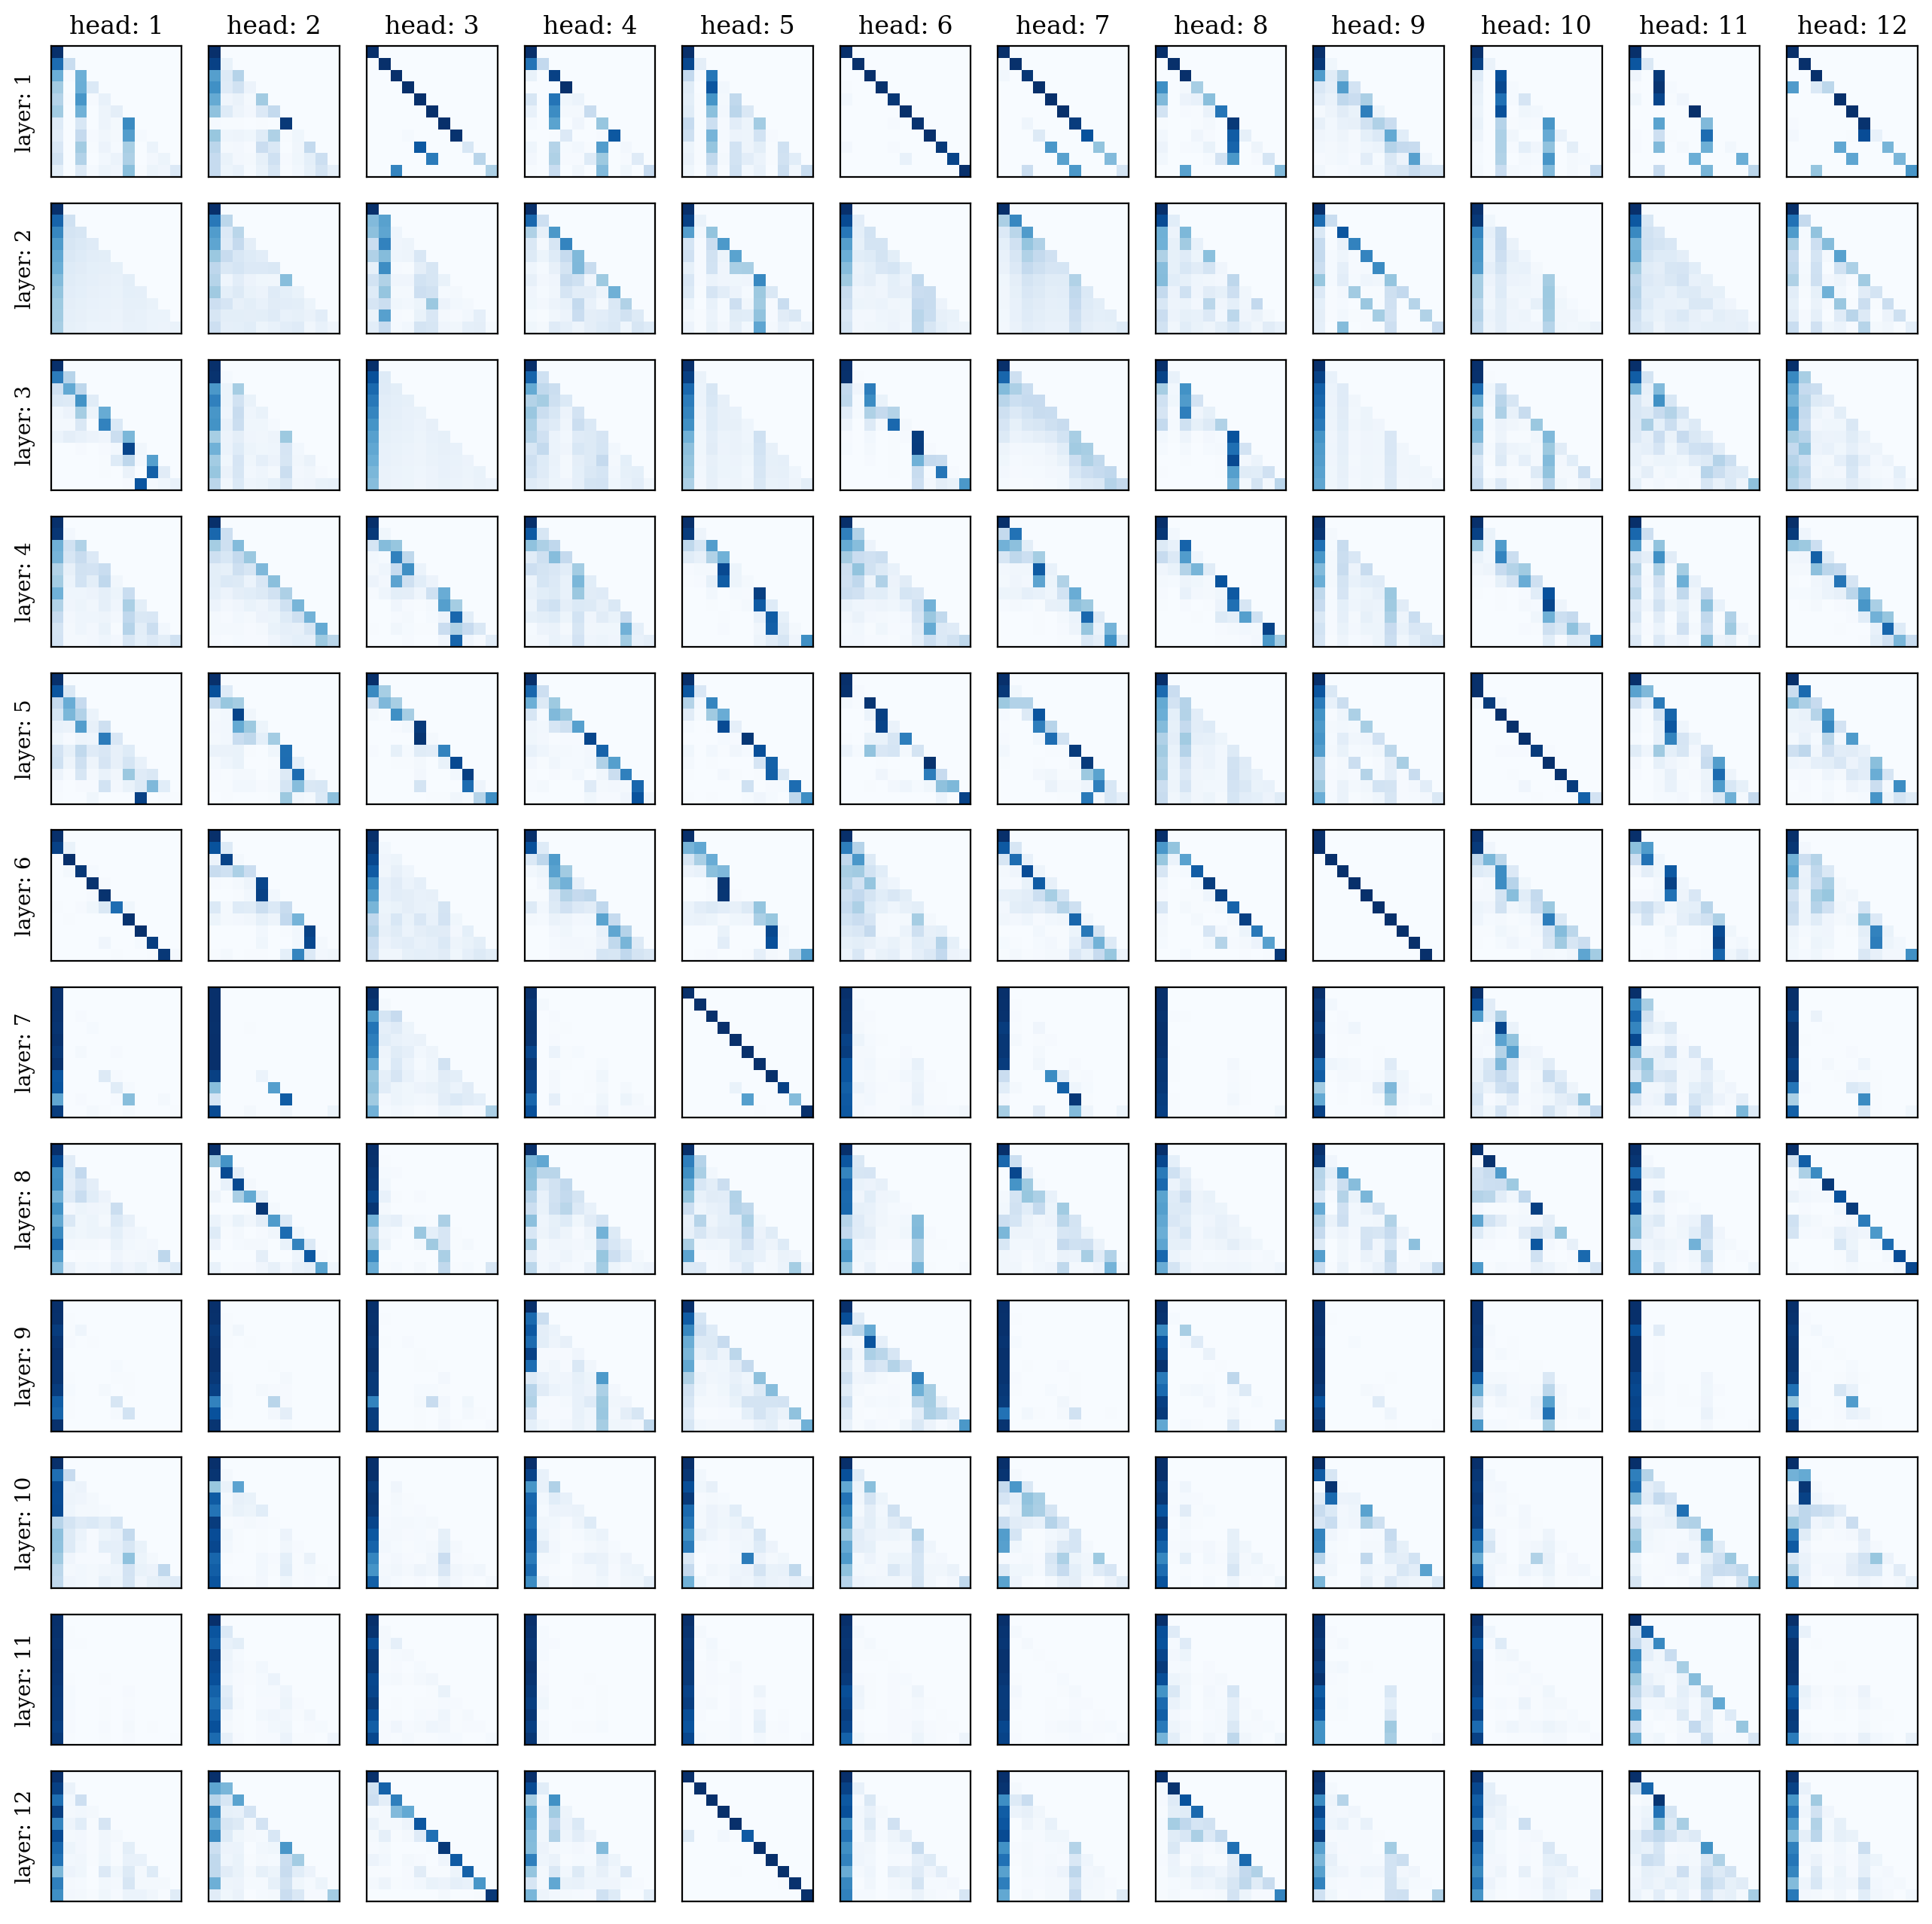
\includegraphics[width=\linewidth]{figures/gpt_neo_attn.png}
    \vspace{2mm}
    % 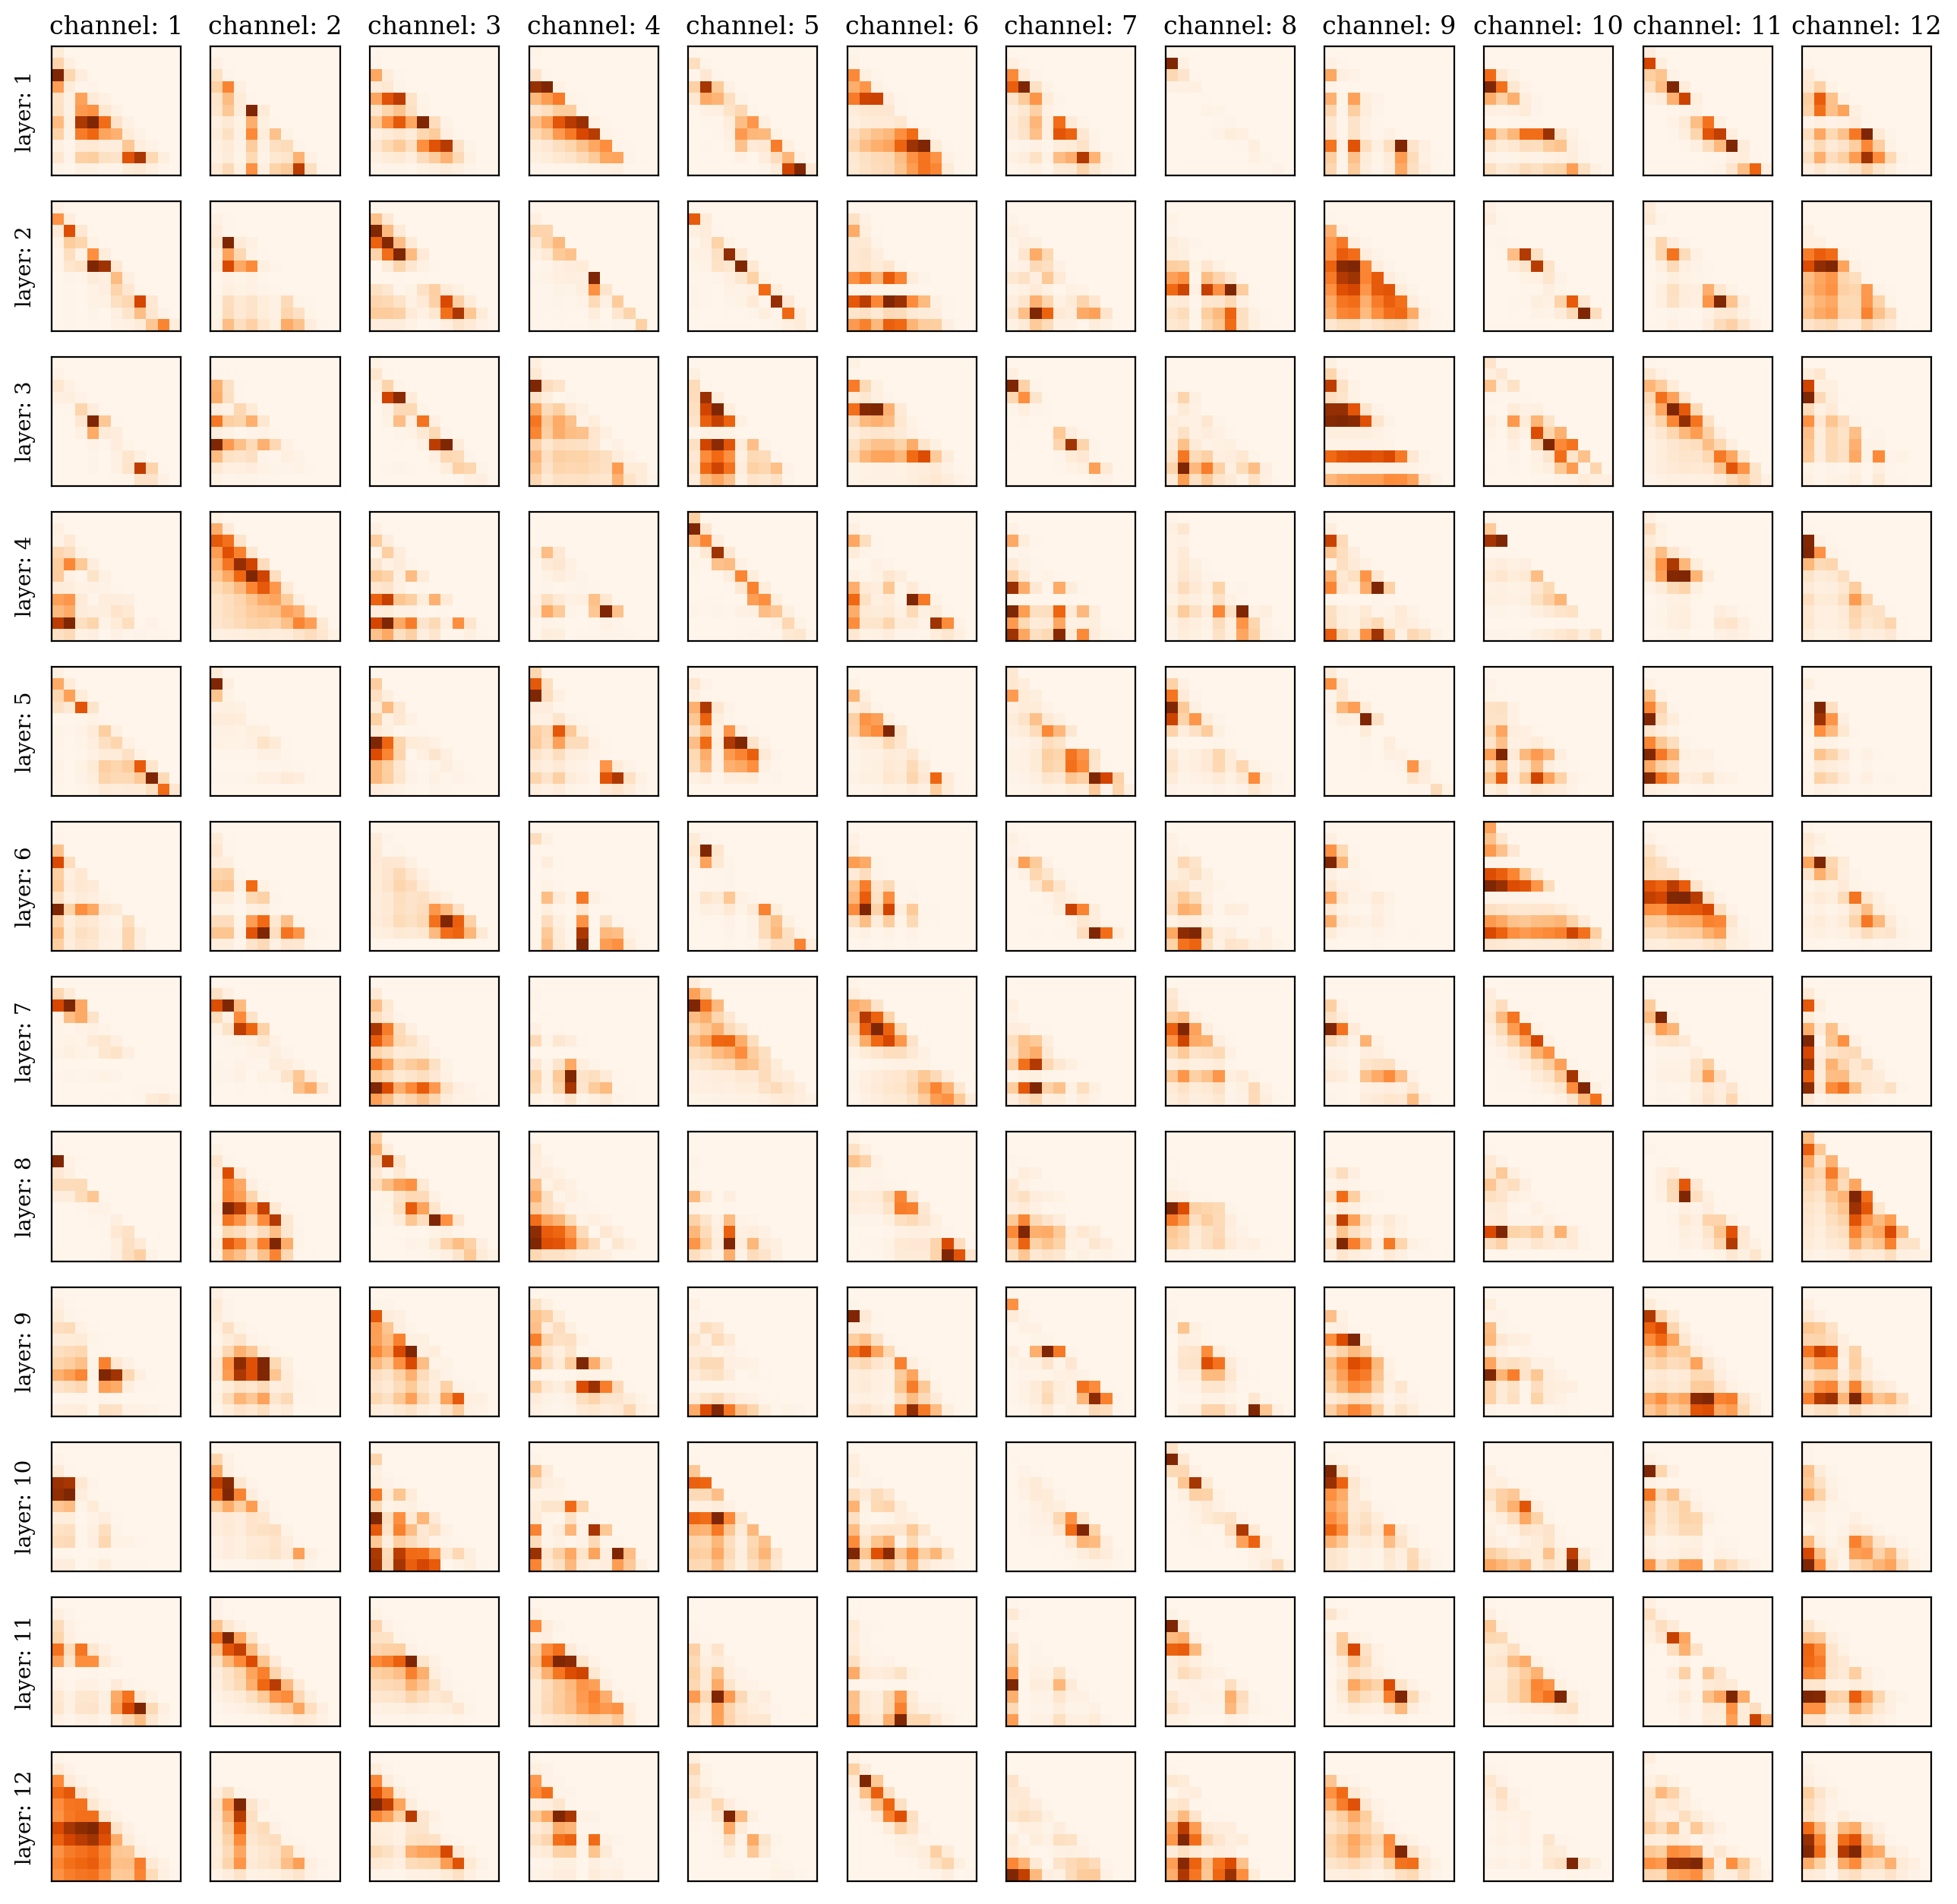
\includegraphics[width=0.6\linewidth]{figures/hyena_mats.png}
    %\caption{\textbf{[Top]}: Attention matrices from a GPTNeo small model. \textbf{[Bottom]}:  Hyena matrices from a {\sf Hyena} small (same model used for SuperGLUE downstream evaluations). "We use the test string "\textit{Attention is all you need. Attention is}". We note that {\sf Hyena} has a different data-controlled matrix for each \textit{channel} i.e. for each dimension in its width, since it does not use heads.}
    \caption{Attention matrices from a GPTNeo small model. "We use the test string "\textit{Attention is all you need. Attention is}".}
    \label{fig:comparisons_1}
\end{figure}
%
\begin{figure}
    \centering
    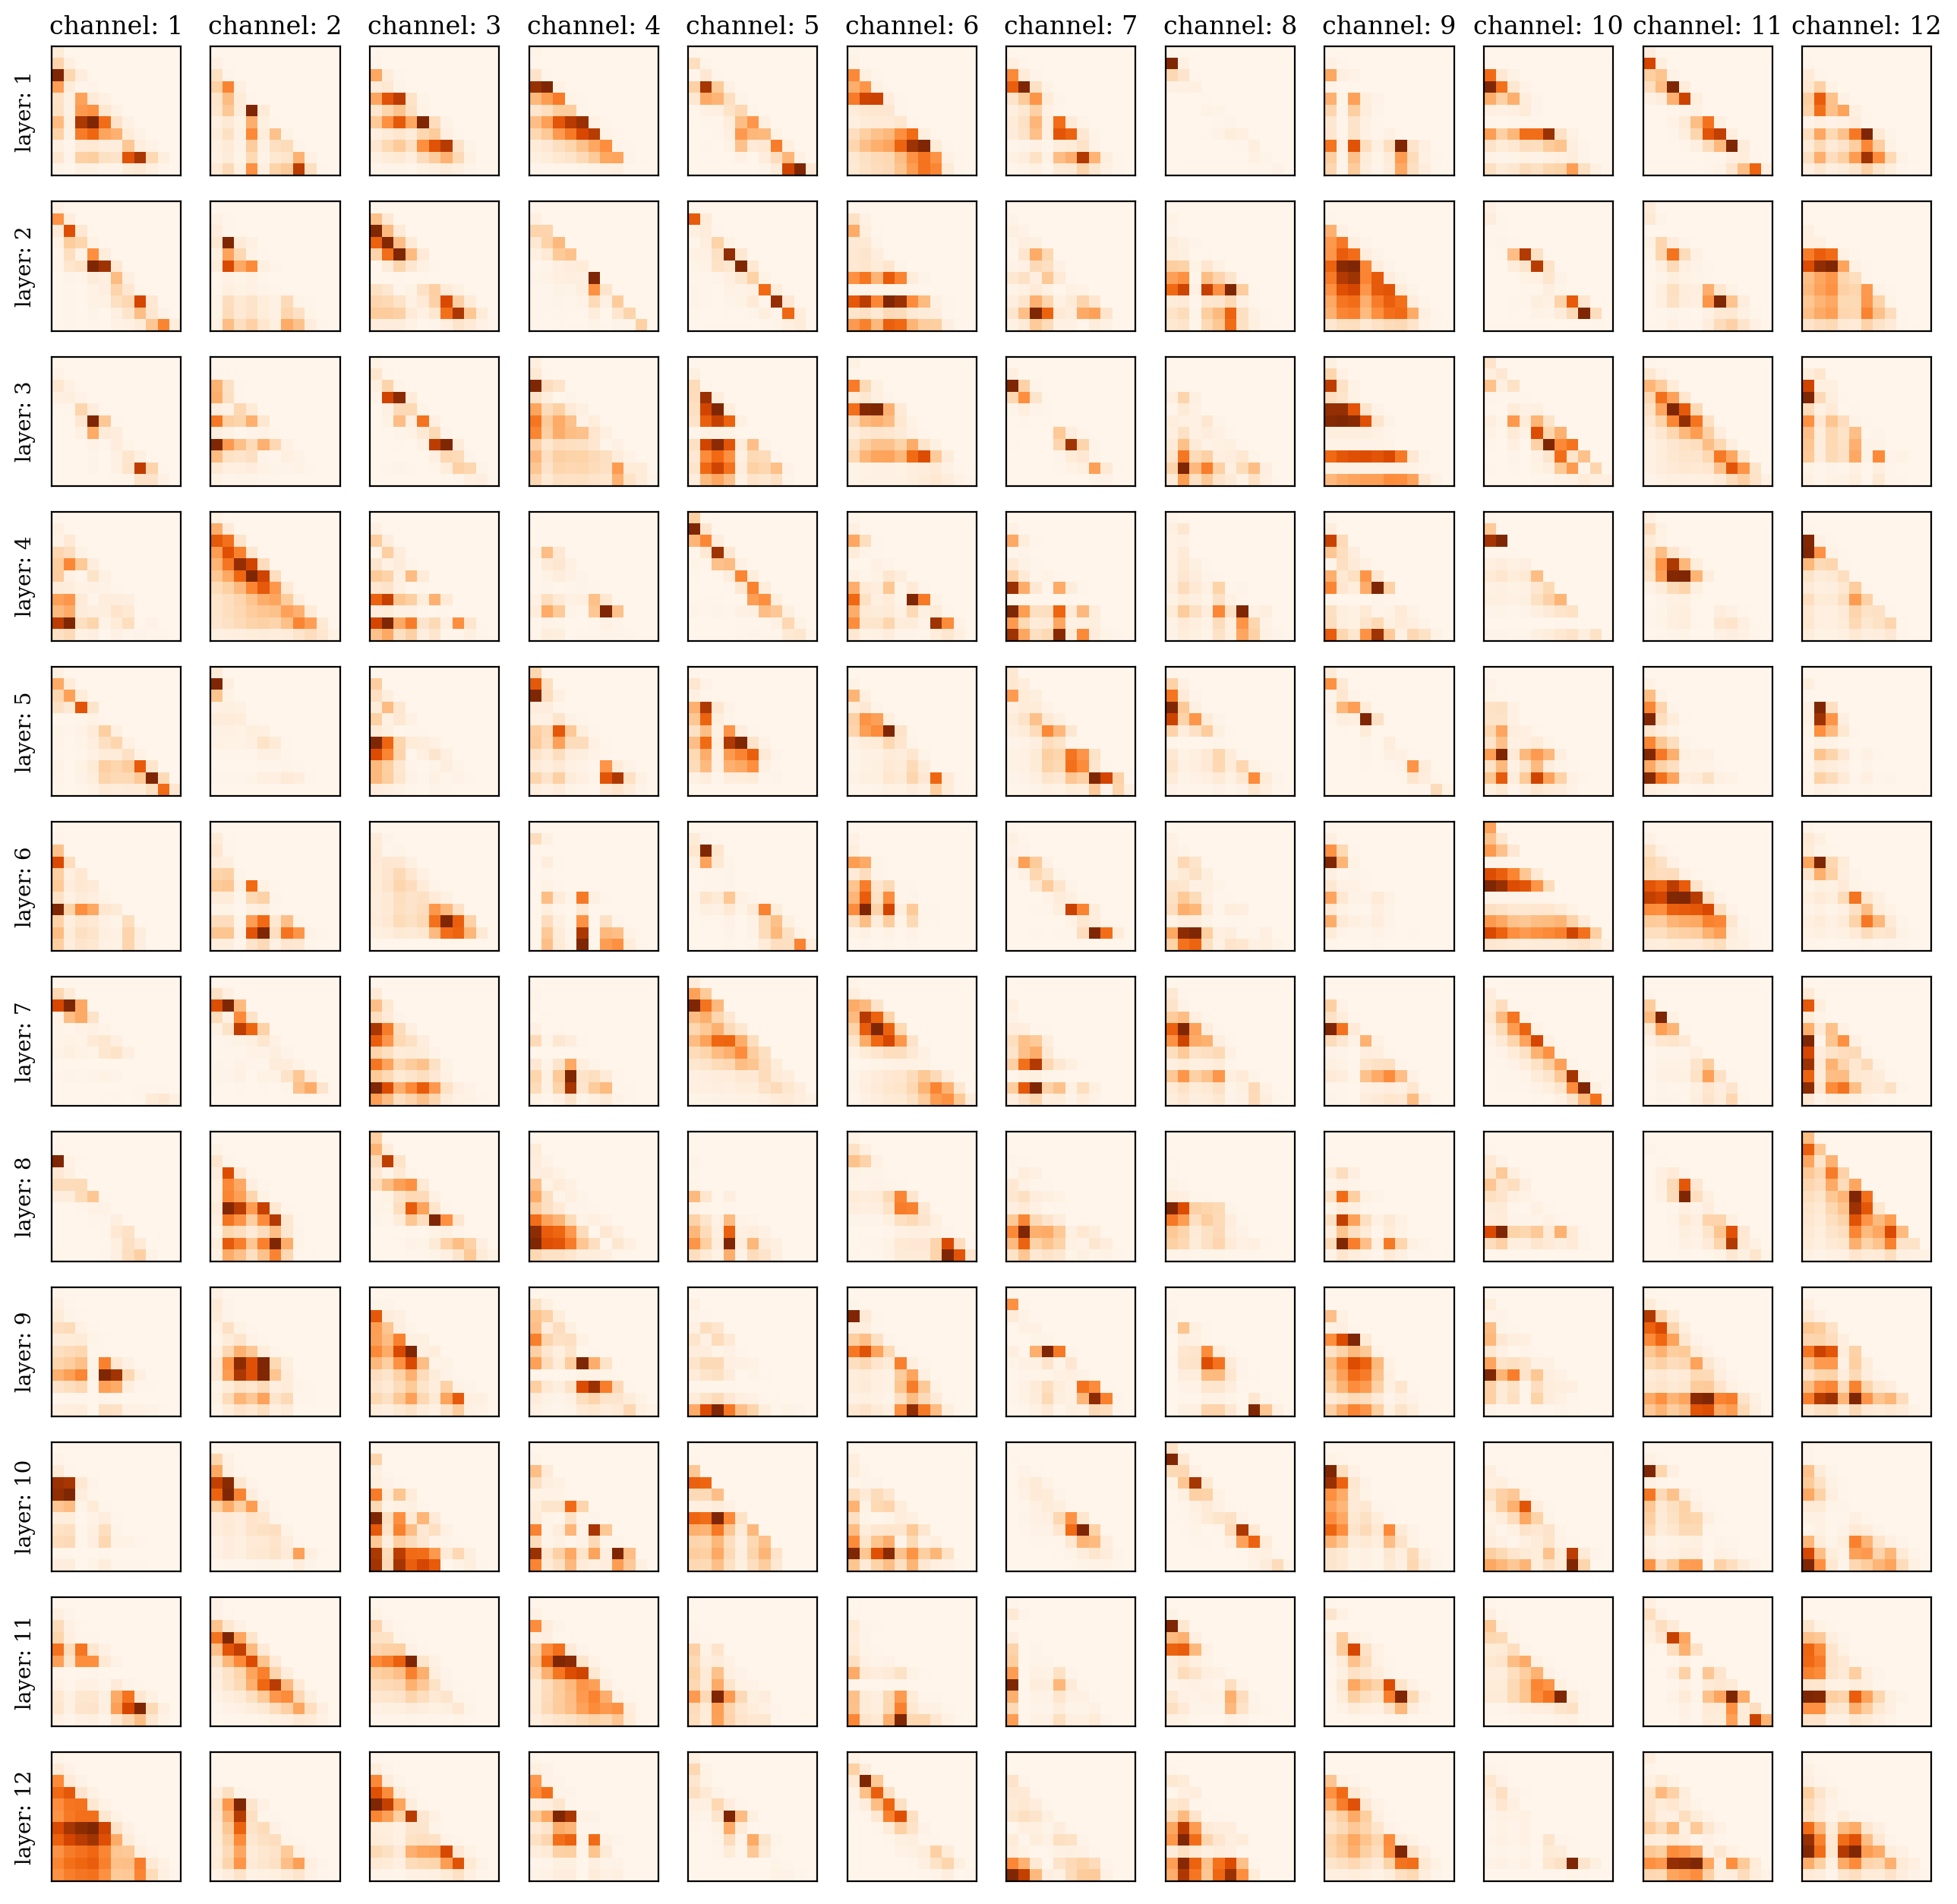
\includegraphics[width=\linewidth]{figures/hyena_mats.png}
    \caption{Hyena matrices from a {\sf Hyena} small (same model used for SuperGLUE downstream evaluations). "We use the test string "\textit{Attention is all you need. Attention is}". We note that {\sf Hyena} has a different data-controlled matrix for each \textit{channel} i.e. for each dimension in its width, since it does not use heads.}
    \label{fig:comparisons_2}
\end{figure}
%

\begin{figure}[h]
    \centering
    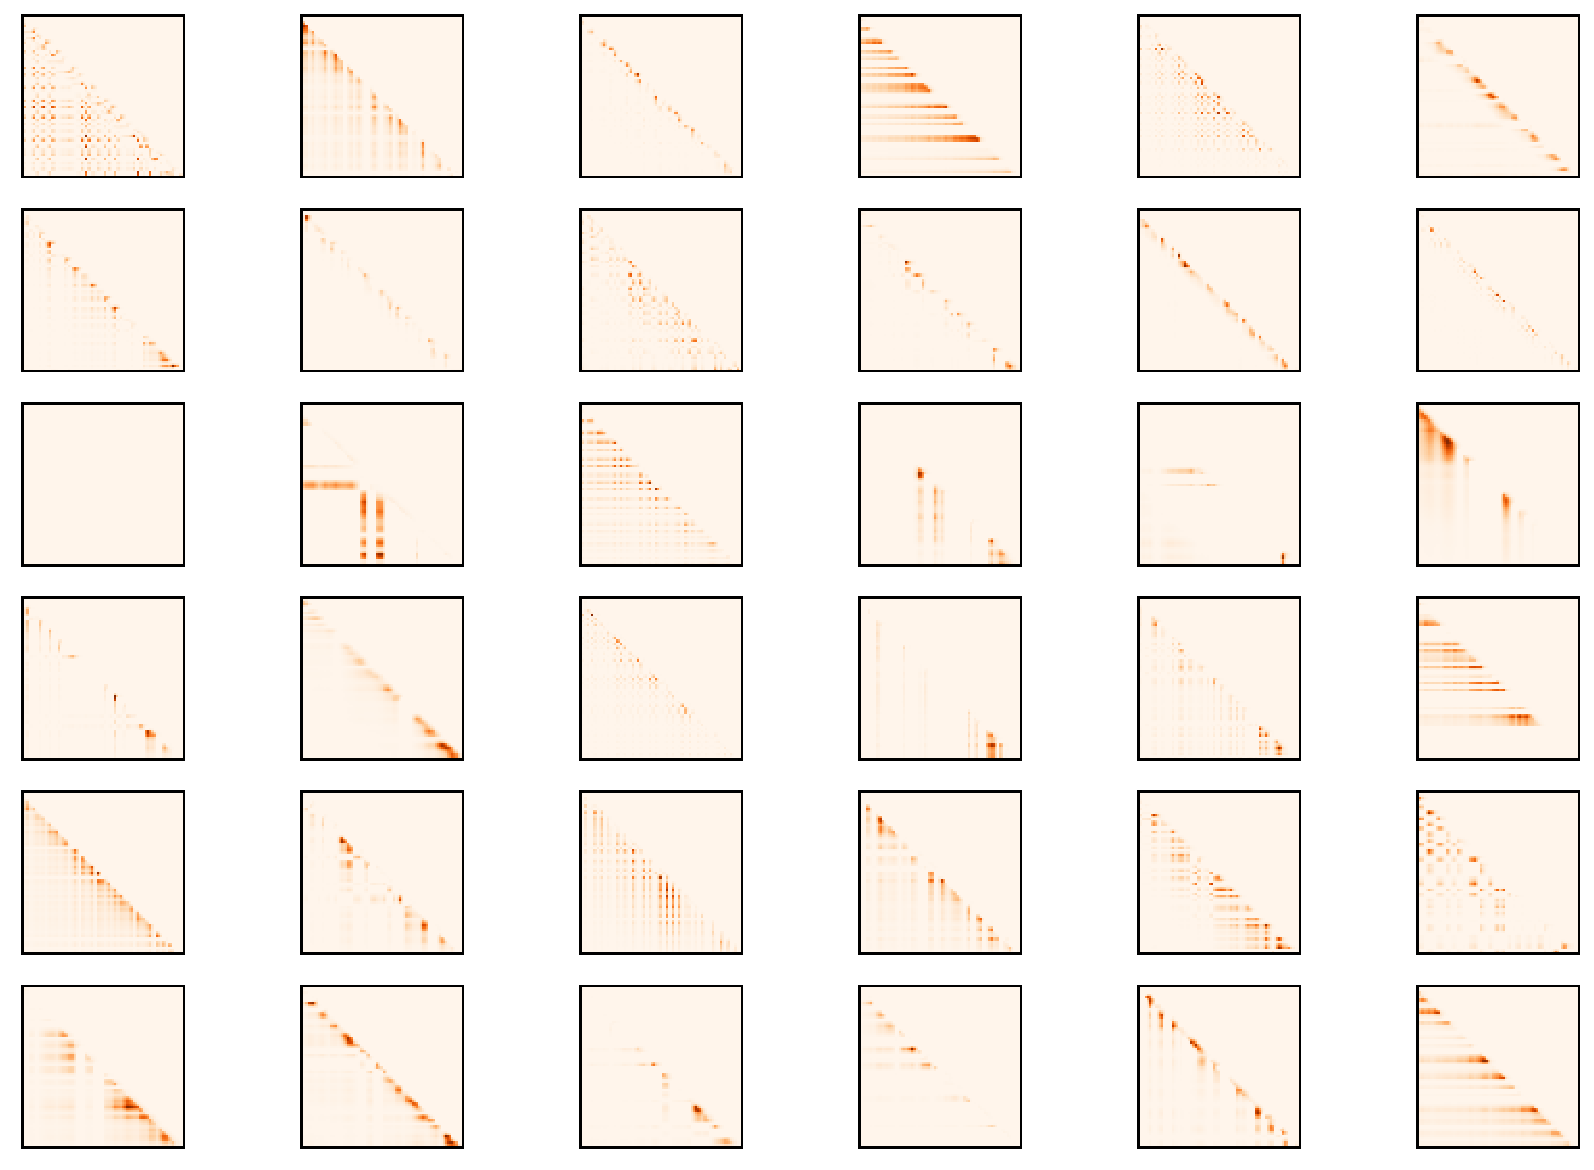
\includegraphics[width=\linewidth]{figures/hyena_doctor.pdf}
    \caption{Data-controlled ${\sf Hyena}$ matrices ($355$M model), activated by the string "\textit{When a doctor doctors a doctor, does the doctor doing the doctoring doctor as the doctor being doctored wants to be doctored or does the doctor doing the doctoring doctor as they want to doctor?}". Rows in the plot are matrices from different layers, columns are matrices from different channels. The operator shows characteristic patterns of attention matrices, without attention.}
    \label{fig:visu}
\end{figure}
\begin{figure}[h]
    \centering
    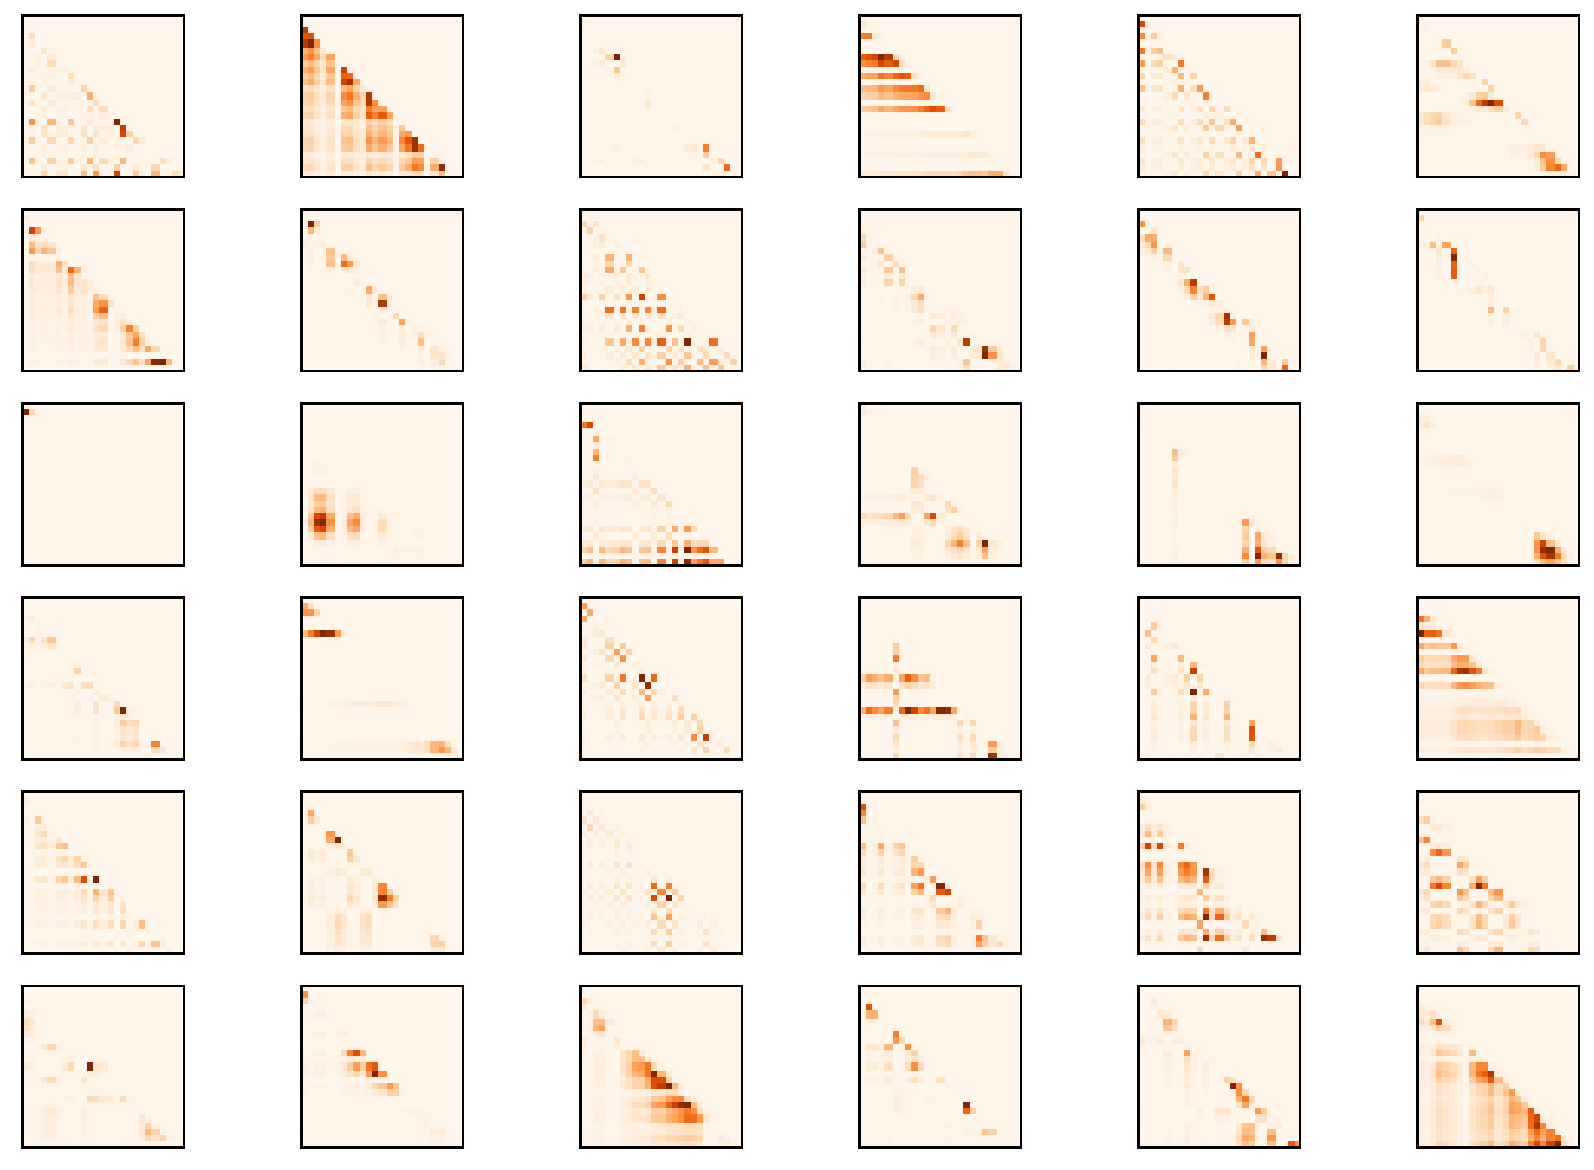
\includegraphics[width=\linewidth]{figures/hyena_dursley.pdf}
    \caption{Data-controlled ${\sf Hyena}$ matrices ($355$M model), activated by the string "\textit{Mrs. Dursley, Mr. Dursley, Dudley Dursley}", from \href{ttps://www.lesswrong.com/posts/j6s9H9SHrEhEfuJnq/causal-scrubbing-results-on-induction-heads}{\textit{Causal scrubbing: results on induction heads}}. Rows in the plot are matrices from different layers, columns are matrices from different channels.}
    \label{fig:visu2}
\end{figure}

\clearpage 

\subsection{Hyena Filters}

Figure \ref{fig:hyena_filters} provides a visualization of {\sf Hyena} long convolution filters at initialization and after training to completion on {\sc The Pile}. 

 We find a substantial performance difference (up to $5\%$ perplexity) between initialization schemes. If the filters at initialization are excessively smooth (see Appendix \ref{app:posemb} for a discussion of positional encoding and activation), the model finds a worse solution and takes longer to converge. Further, we observe initialization schemes that regularize filters towards typical filters learned at convergence to decrease performance. These observations are in line with performance gaps between convolution parametrization schemes discussed in main text and Appendix \ref{app:icl}. In particular, the performance improvements obtained via {\sf Hyena} filters could be due to easier optimization in the space of convolutional filters.


%
 At convergence, {\sf Hyena} learns a collection of lower-order filters with a similar structure, which can be exploited to further speed up inference after training. 

 
\begin{figure}
    \centering
    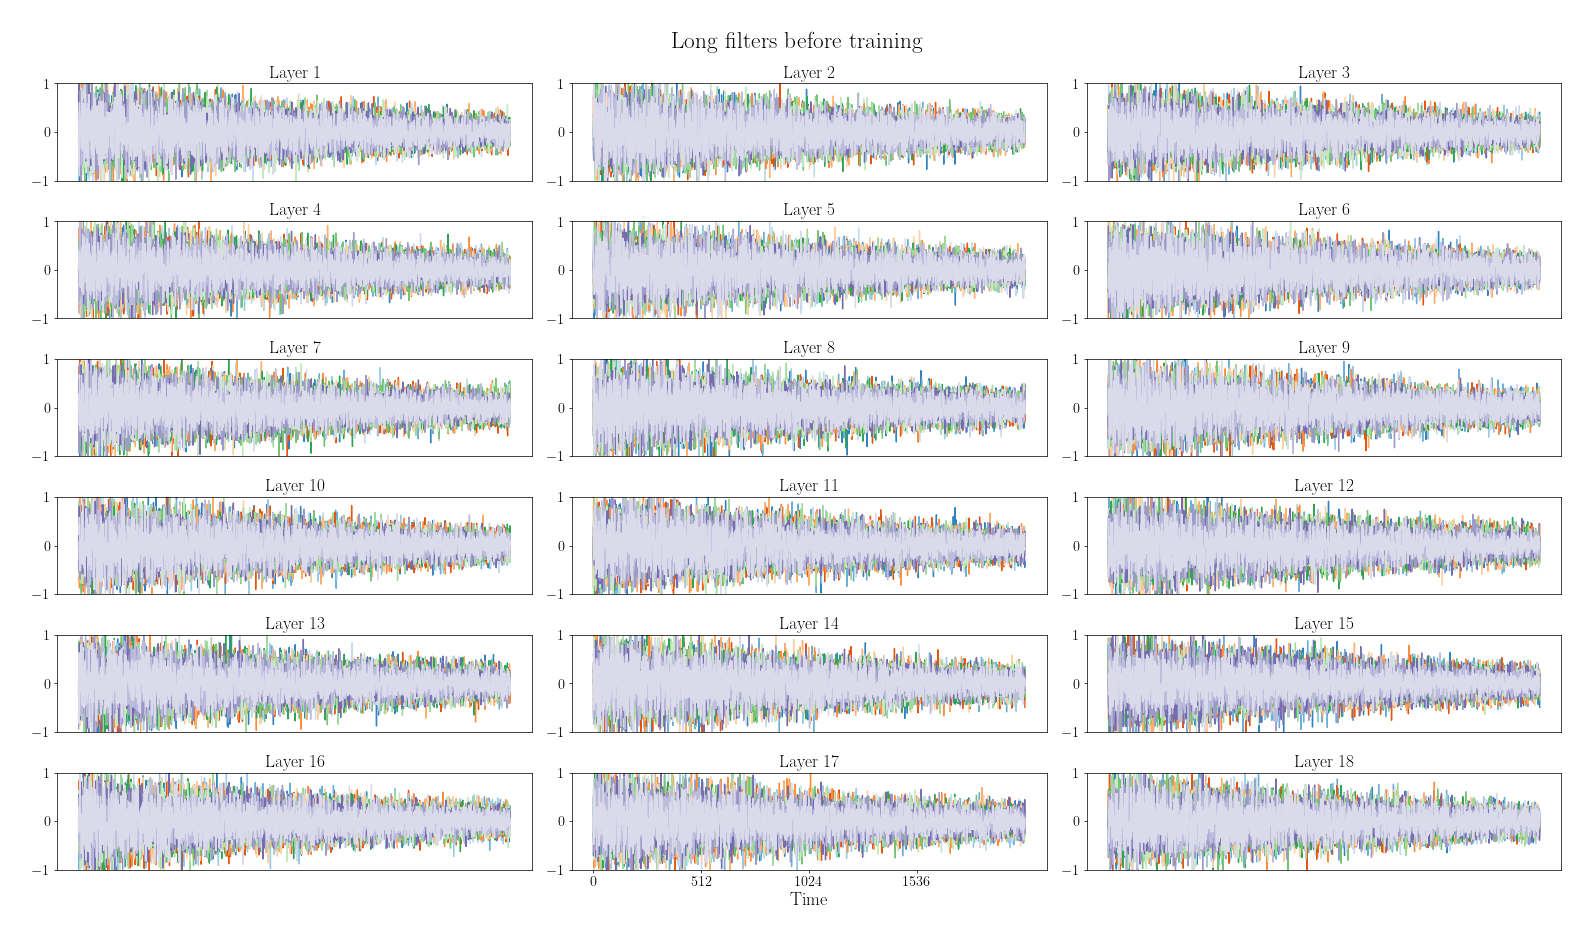
\includegraphics[width=0.99\linewidth]{figures/long_filters_init.png}
    \vspace{2mm}
    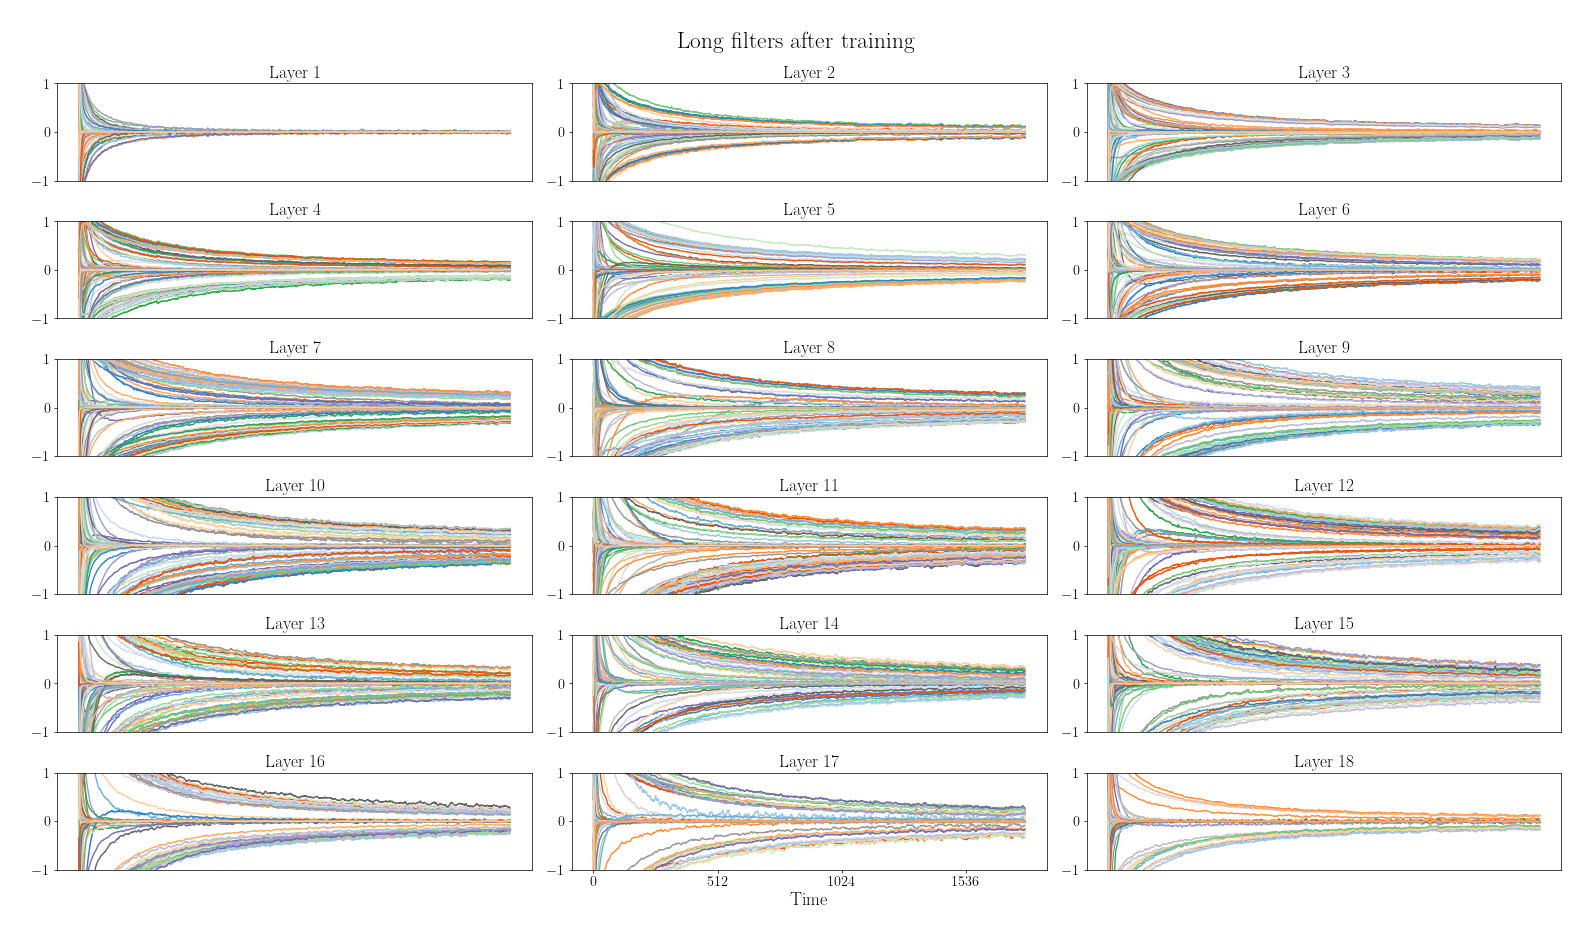
\includegraphics[width=0.99\linewidth]{figures/long_filters.png}
    \caption{\textbf{[Top]}: Long convolution {\sf Hyena} filters at initialization ($153$M parameters, $18$ layer model). \textbf{[Bottom]}: Filters after training for $130$ billion tokens on {\sc The Pile}.}
    \label{fig:hyena_filters}
\end{figure}

\subsection{Positional Encoding and Filters Initialization}\label{app:posemb}
%
The positional encoding chosen for the $\sf Hyena$ filters is a truncated complex exponential basis. Specifically, with $\rho_k(t) = e^{i2\pi kt/L}$ for $k=0,\dots K-1$, the positional encoding is defined as a map from $\R$ to $\R^{2K+1}$ such that
%
\[
    {\sf PositionalEncoding}(t) = 
    \begin{bmatrix}
        t&
        \mathfrak{R}[\rho_0](t)&
        \cdots&
        \mathfrak{R}[\rho_{K-1}](t)&
        \mathfrak{I}[\rho_0](t)&
        \cdots&
        \mathfrak{I}[\rho_{K-1}](t)
    \end{bmatrix}
\]
%
where $\mathfrak{R}[\cdot]$, $\mathfrak{I}[\cdot]$ denote the real and imaginary part of their argument, respectively. In the main text, we use $D_e = 2K + 1$ to denote the size of a positional encoding with $K$ features. The number of features of the positional encoding has an impact on the filter initialization and training performances. In particular, we show how $K$ leads to a preconditioning of the spectrum of the filter at initialization. Figures~\ref{fig:pos_enc_17_1},~\ref{fig:pos_enc_65_1},~\ref{fig:pos_enc_128_1} display the initialized filters (with no $\sf Window$ function) for different values of $K$ ($\{8, 32, 64\}$) for $L=128$ and frequency $\omega_a$ of sinusoidal activation $\sigma(\cdot) = \sin(\omega_a \cdot)$ set to 1. We notice how the choice of $K$ induces a bias in the modeled frequencies at initialization. Specifically the filters resemble low-pass filters with a cut-off frequency of approximatively $2K + 1$. 

This cut-off frequency is strongly related to the \textit{smoothness} of the filter; as previously mentioned, we empirically observe better training dynamics of filters initialized to be non-smooth, i.e. with a rich high-frequency content. While we can achieve good initializations by increasing $K$, this results in larger $\sf FFN$s (its input dimension is $2K + 1$, i.e. the number of positional encoding features) which come with a higher parameter count. A more efficient solution is to increase the frequency $\omega_a$ of the sinusoidal activation. Figure~\ref{fig:pos_enc_17_10} show how with $K=8$ we can cover the full spectrum simply by setting $\omega_a=10$. 

%
\begin{figure}
    \centering
    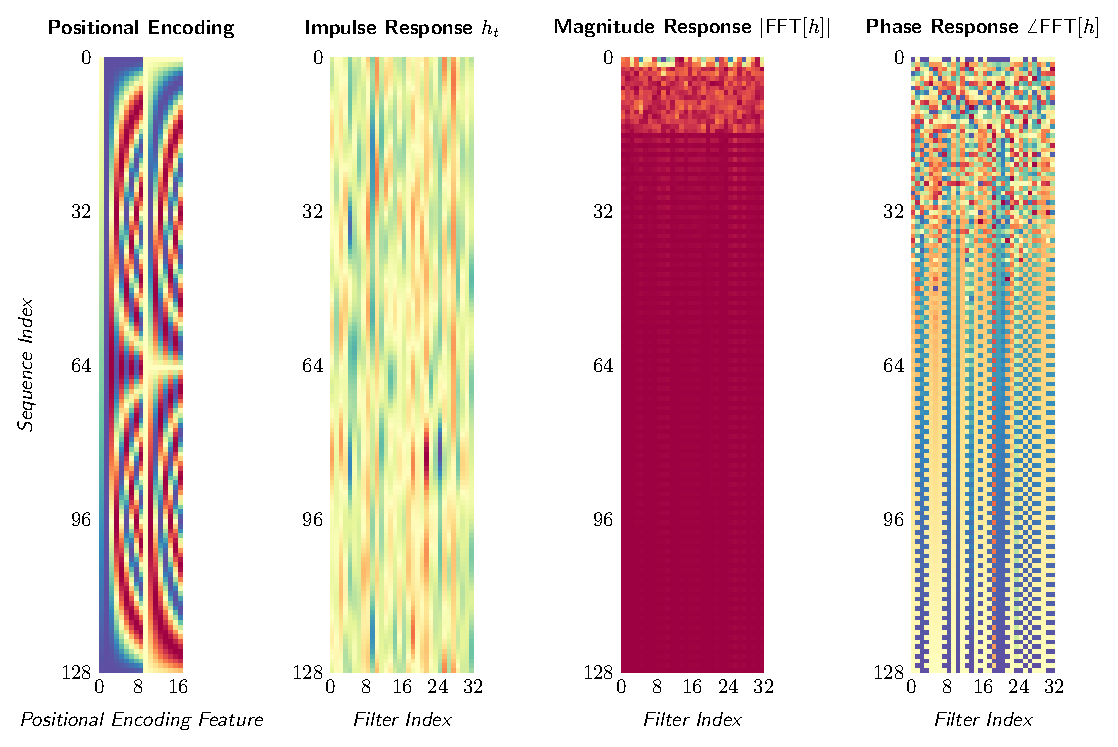
\includegraphics[width=.8\linewidth]{figures/pos_enc_17_sin_freq_1.pdf}
    \caption{$\sf Hyena$ filters at initialization with 17 positional encoding features $K=8$.}
    \label{fig:pos_enc_17_1}
\end{figure}
\begin{figure}
    \centering
    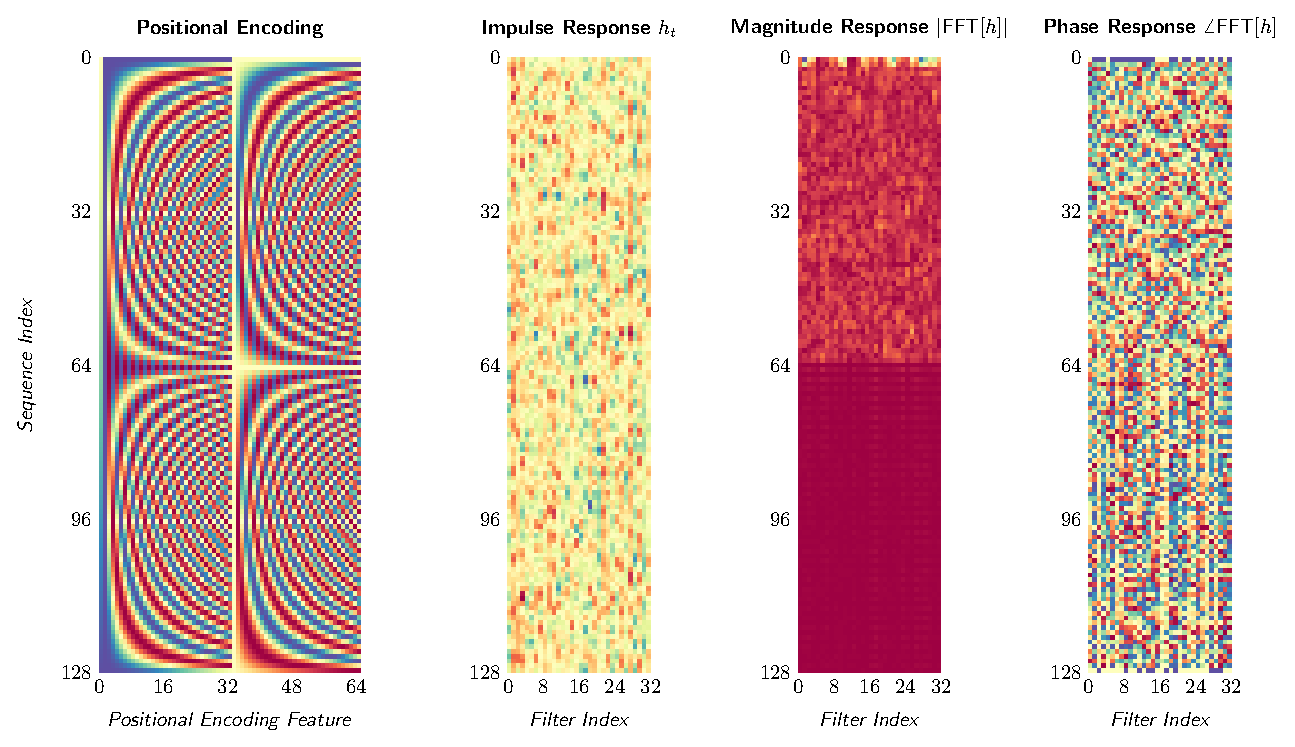
\includegraphics[width=.8\linewidth]{figures/pos_enc_65_sin_freq_1.pdf}
    \caption{$\sf Hyena$ filters at initialization with 65 positional encoding features $K=32$.}
    \label{fig:pos_enc_65_1}
\end{figure}
\begin{figure}
    \centering
    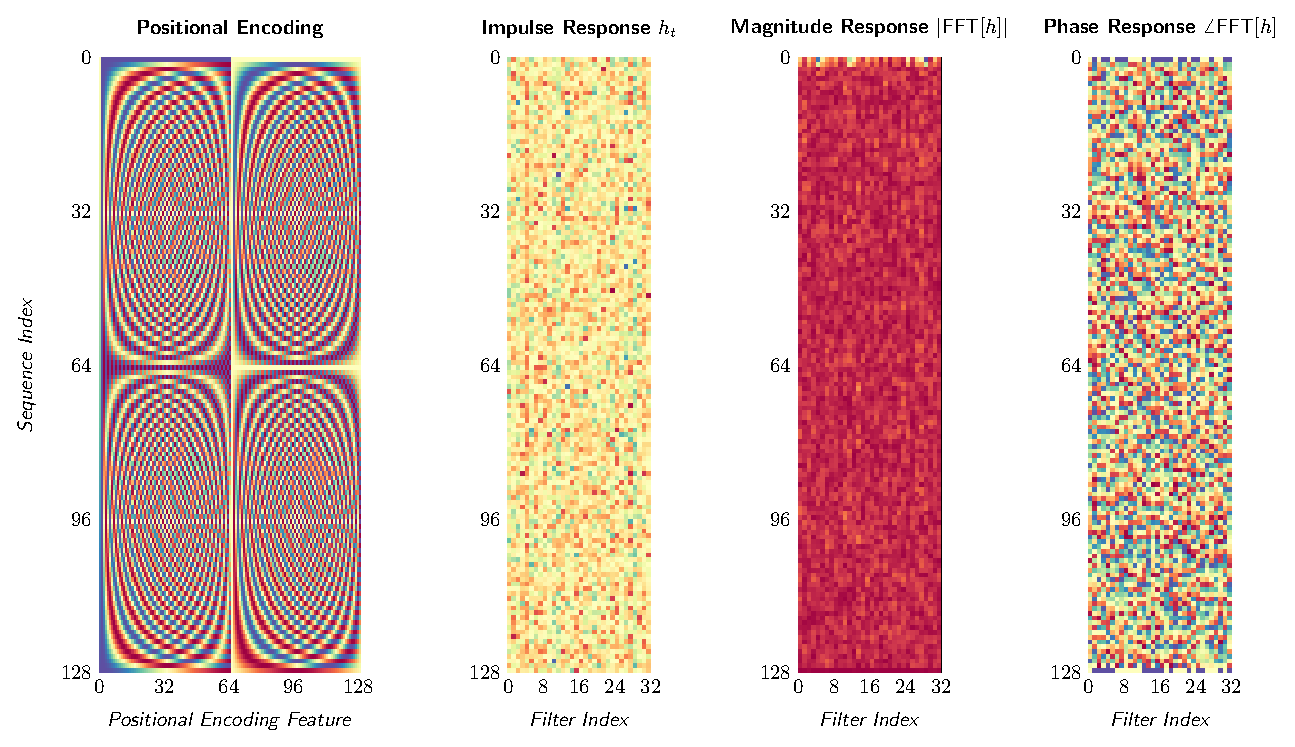
\includegraphics[width=.9\linewidth]{figures/pos_enc_129_sin_freq_1.pdf}
    \caption{$\sf Hyena$ filters at initialization with 65 positional encoding features $K=64$.}
    \label{fig:pos_enc_128_1}
\end{figure}
\begin{figure}
    \centering
    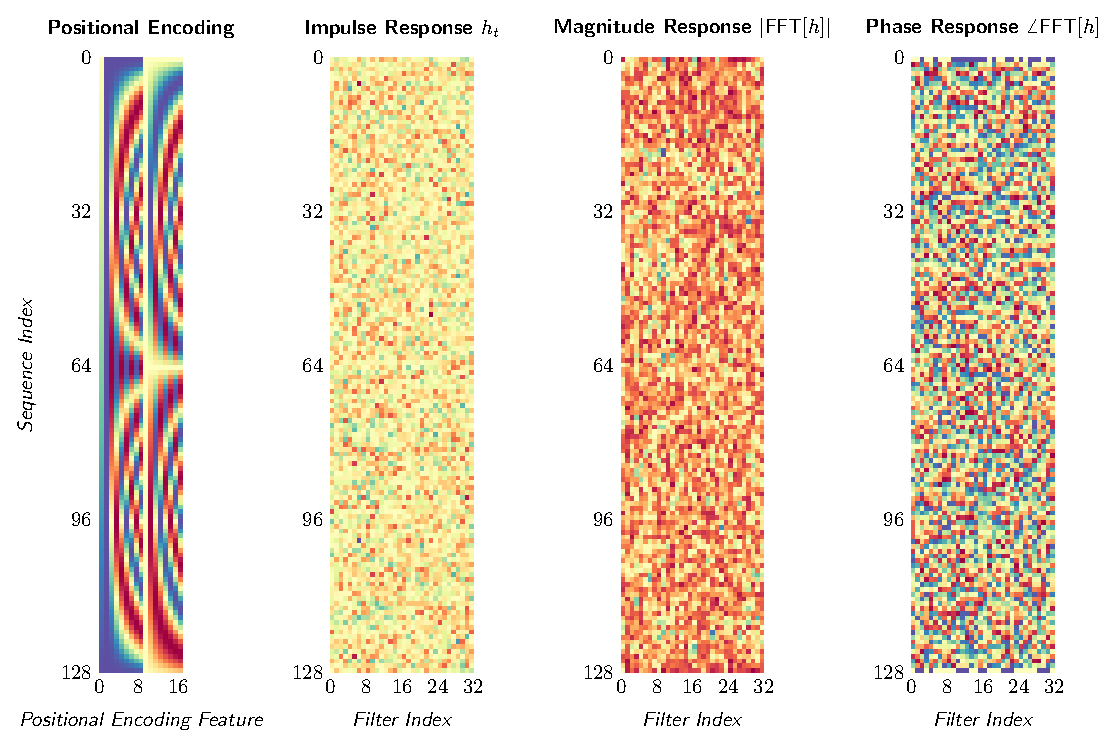
\includegraphics[width=.9\linewidth]{figures/pos_enc_17_sin_freq_10.pdf}
    \caption{$\sf Hyena$ filters at initialization with 17 positional encoding features $K=8$ and frequency of sinusodial activation set to 10.}
    \label{fig:pos_enc_17_10}
\end{figure}

\clearpage

\subsection{Downstream Examples}

\paragraph{MultiRC}
%

We report examples of downstream evaluation of small models on the MultiRC question-answering task. We report answers of small {\sf Hyena} (153M, trained for $130$B tokens on {\sc The Pile}) and the public checkpoint RWKV-v4 \citep{PENG_RWKV-LM_2021} ($169$M, trained for $332$B tokens on {\sc The Pile}). We select randomized examples with indices being powers of $2$.
%
Alignment of {\sf Hyena}'s responses to the task format is greatly improved by providing few-shot examples in the prompt, which may be a promising sign for larger models based on the proposed attention-free architecture.
Each example shows responses for specific examples in the validation set (example indices are listed at the beginning of each example).

\begin{tcolorbox}[sharp corners]
    {\tt MultiRC} index: 2, 4 \\ 
    
    \small {\tt \textbf{Passage:} What causes a change in motion? The application of a force. Any time an object changes motion, a force has been applied. In what ways can this happen? Force can cause an object at rest to start moving. Forces can cause objects to speed up or slow down. Forces can cause a moving object to stop. Forces can also cause a change in direction. In short, forces cause changes in motion. The moving object may change its speed, its direction, or both. We know that changes in motion require a force. We know that the size of the force determines the change in motion. How much an object's motion changes when a force is applied depends on two things. It depends on the strength of the force. It also depends on the object's mass. Think about some simple tasks you may regularly do. You may pick up a baseball. This requires only a very small force.} \\ 
    
    {\tt \textbf{Question:} Based on the previous passage, Would the mass of a baseball affect how much force you have to use to pick it up? Is "Less the mass, less the force applied" a correct answer?} \\

    {\tt \textbf{Answer:} Yes} \\ 

    {\tt {\color{red!80} RWKV zero-shot}: The mass of a baseball depends on the force applied. if the mass of the baseball is small, the force applied is small.}  \\ 

    {\tt {\color{blue!80}Hyena zero-shot}: Yes it is.}  \\

    {\tt {\color{red!80} RWKV few-shot}: The mass, less the force applied, is a more important force. it is the force that changes the mass of a baseball.} \\

    {\tt {\color{blue!80}Hyena few-shot}: Yes.} 

    \vspace{1cm}
    
     {\tt \textbf{Question:} Based on the previous passage, What do you apply to an object to make it move or stop? Is "Strength" a correct answer?} \\

    {\tt \textbf{Answer:} No} \\    

    {\tt {\color{red!80} RWKV zero-shot}: The force applied to the object is the force applied to the object.}  \\ 

    {\tt {\color{blue!80}Hyena zero-shot}: Yes.}  \\

    {\tt {\color{red!80} RWKV few-shot}: The force applied to a baseball is a force. it is a force that is applied to a baseball.} \\

    {\tt {\color{blue!80}Hyena few-shot}: Yes.} 
\end{tcolorbox}



\begin{tcolorbox}[sharp corners]
    {\tt MultiRC} index: 32, 64 \\ 
    
    \small {\tt \textbf{Passage:} The film opens with Sunita, a medical student, and her friends working on a project about the human brain. She wants to investigate the curious case of Sanjay Singhania, a notable city businessman, who is reported to have anterograde amnesia.  Her professor denies access to Sanjay's records as it is currently under criminal investigation.  Sunita, nonetheless, decides to investigate the matter herself.  Sanjay is introduced as he brutally murders a man. He takes a Polaroid picture of the man, and writes on it ``done''.  It is revealed that Sanjay has anterograde amnesia where he loses his memory every 15 minutes.  Sanjay uses a system of photographs, notes, and tattoos on his body to recover his memory after each cycle.  It is revealed that Sanjay is ultimately out to avenge the death of his sweetheart Kalpana, and that he is systematically killing the people who were responsible for it.  His main target is ``Ghajini'', a notable social personality in the city. Police Inspector Arjun Yadav, on the case of the serial murders, tracks Sanjay down to his flat and attacks and disables him. Yadav finds two diaries where Sanjay has chronicled the events of 2005 and 2006 . The film flashes back to 2005 as Yadav reads the diary. Sanjay Singhania is shown as the owner of the Air Voice mobile telephone company. In the course of his business, Sanjay sends his men to meet Kalpana, a struggling model, about putting up a billboard above her apartment. The owner of Kalpana's advertising firm misinterprets this as a romantic advance, and in view of a possible lucrative Air Voice ad campaign and other benefits, encourages Kalpana to accept the overture.} \\ 
    
    {\tt \textbf{Question:} Based on the previous passage, Why did Sanjay murder a man? Is "Sanjay" a correct answer?} \\

    {\tt \textbf{Answer:} Yes} \\ 

    {\tt {\color{red!80} RWKV zero-shot}: The answer is "Sanjay".}  \\ 

    {\tt {\color{blue!80}Hyena zero-shot}: The answer is}  \\

    {\tt {\color{red!80} RWKV few-shot}: The question is not about Sanjay's death.} \\

    {\tt {\color{blue!80}Hyena few-shot}: No.}  \\ 

    \vspace{1cm}

      {\tt \textbf{Question:} Based on the previous passage, Every 15 minutes, Sanjay goes through what process, Which frustrates his attempts to avenge the death of his sweetheart? Is "He forgets about facts" a correct answer?} \\

    {\tt \textbf{Answer:} Yes} \\    

    {\tt {\color{red!80} RWKV zero-shot}: Yes, it is a correct answer..}  \\ 

    {\tt {\color{blue!80}Hyena zero-shot}: The answer is.}  \\

    {\tt {\color{red!80} RWKV few-shot}: The answer is "yes".} \\

    {\tt {\color{blue!80}Hyena few-shot}: The answer is "yes.}    
\end{tcolorbox}

\begin{tcolorbox}[sharp corners]
    {\tt MultiRC} index: 128 \\ 
    
    \small {\tt \textbf{Passage:} In 1863, Alexander II re-convened the Diet of Finland and initiated several reforms increasing Finland\'s autonomy from Russia including establishment of its own currency, the markka. Liberation of business led to increased foreign investment and industrial development. Finland also got its first railways, separately established under Finnish administration. Finally, the elevation of Finnish from a language of the common people to a national language equal to Swedish opened opportunities for a larger proportion of the society. Alexander II is still regarded as "The Good Tsar" in Finland. These reforms could be seen as results of a genuine belief that reforms were easier to test in an underpopulated, homogeneous country, than in the whole of Russia. They may also be seen as a reward for the loyalty of its relatively western-oriented population during the Crimean War and during the Polish uprising. Encouraging Finnish nationalism and language can also be seen as an attempt to dilute ties with Sweden.} \\ 
    
    {\tt \textbf{Question:} Based on the previous passage, Alexander II is considered what in Finland since 1863? Is "The good tsar" a correct answer?} \\

    {\tt \textbf{Answer:} Yes} \\ 

    {\tt {\color{red!80} RWKV zero-shot}: The correct answer is "yes".}  \\ 

    {\tt {\color{blue!80}Hyena zero-shot}: Yes, the question is correct.}  \\

    {\tt {\color{red!80} RWKV few-shot}: The Finnish language is a language of the people.} \\

    {\tt {\color{blue!80}Hyena few-shot}: Yes.} 
\end{tcolorbox}


\begin{tcolorbox}[sharp corners]
    {\tt MultiRC} index: 1024 \\ 
    
    \small {\tt \textbf{Passage:} Einstein and Maric married in January 1903. In May 1904, the couple's first son, Hans Albert Einstein, was born in Bern, Switzerland. Their second son, Eduard, was born in Zurich in July 1910. In 1914, the couple separated; Einstein moved to Berlin and his wife remained in Zurich with their sons. They divorced on 14 February 1919, having lived apart for five years. Eduard, whom his father called "Tete" (for petit), had a breakdown at about age 20 and was diagnosed with schizophrenia. His mother cared for him and he was also committed to asylums for several periods, including full-time after her death. The marriage with Maric does not seem to have been very happy. In letters revealed in 2015, Einstein wrote to his early love, Marie Winteler, about his marriage and his still strong feelings for Marie. In 1910 he wrote to her that "I think of you in heartfelt love every spare minute and am so unhappy as only a man can be" while his wife was pregnant with their second child. Einstein spoke about a "misguided love" and a "missed life" regarding his love for Marie. Einstein married Elsa Lowenthal on 2 June 1919, after having had a relationship with her since 1912. She was a first cousin maternally and a second cousin paternally. In 1933, they emigrated to the United States. In 1935, Elsa Einstein was diagnosed with heart and kidney problems; she died in December 1936.} \\ 
    
    {\tt \textbf{Question:} Based on the previous passage, How much time passed, after Albert Einstein's father divorced his mother, that he re-married? Is "3 months and 18 days" a correct answer?} \\

    {\tt \textbf{Answer:} Yes} \\ 

    {\tt {\color{red!80} RWKV zero-shot}: Albert Einstein was born on 3 march 1916 in Gerlin, Germany. he was the son of a German doctor and a german woman.}  \\ 

    {\tt {\color{blue!80}Hyena zero-shot}: "3 months and 18 days"}  \\

    {\tt {\color{red!80} RWKV few-shot}: It is not a correct answer. The exact date is not known.} \\

    {\tt {\color{blue!80}Hyena few-shot}: Yes, according to the previous passage.} 
\end{tcolorbox}

